\section{Einleitung}

\subsection{Definition Smart Home}
\subsection{Fragestellungen} % TODO better title

% monetarisierung von smart home produkten
% beispiele zu existierenden systemen

\section{Evaluation}

\subsection{Internet of Things} % TODO better title

% Abgrenzung iot / smart home

\subsection{Systembeschreibung}

Aschendorf beschreibt den Aufbau von Smart Home Systemen als hierarchisches System.
\autoref{fig:automatisierungspygramide} zeigt die drei Ebenen der Automatisierungspyramide nach Aschendorf:
Die \textit{Feldbusebene}, die \textit{Automatisierungsebene} und die \textit{Leitebene}. \myfootcite[Vgl.][59]{aschendorf14}

\begin{figure}[ht]
	\centering
	\caption{Automatisierungspyramide nach Aschendorf}
	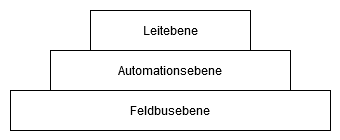
\includegraphics[scale=0.8]{Automatisierungspyramide_nach_Aschendorf}
	\caption*{\footnotesize{Quelle: Eigene Darstellung.}}
	\label{fig:automatisierungspygramide}
\end{figure}

\subsubsection{Feldbusebene}

Die Feldbusebene besteht aus sämtlichen eingebauten Systemkomponenten, also Gateways, welche verschiedene Systeme verbinden, Sensoren, welche z.B. Temperatur und Luftfeuchtigkeit überwachen, und Aktoren, wie z.B. Glühbirnen.
In der selben Ebene finden sich auch die Verbindungen der oben genannten Geräte wieder.
So ist die Feldbusebene in sich bereits funktional und direkt nutzbar.
Es kann z.B. der Sensor \textit{Lichtschalter 3} ausgelöst werden, welcher den Aktor \textit{Deckenlampe Wohnzimmer} aktiviert.\myfootcite[Vgl.][66-67]{aschendorf14}

\subsubsection{Automatisierungsebene}

Geräte übergreifende Automatisierungen werden in der Automatisierungsebene implementiert.
Dies wird durch einfache Controller oder programmierbare Mikrocomputer realisiert.
Nach der Änderung von Zuständen, wie z.B. der aktuellen Zeit, die Anwesenheit eines Bewohners oder die Temperatur eines Raumes, passt sich das Smart Home System mit dieser zusätzlichen Ebene nun nach vorgegebenen Regeln autonom an.\myfootcite[Vgl.][67-68]{aschendorf14}

\subsubsection{Leitebene}

Die Leitebene widmet sich der Interaktion des Smart Home Systems mit dessen Bewohnern.
Es lässt sich die Interaktion teilen in Eingaben und Ausgaben.
Zu den Eingaben zählen Befehle, die z.B. über Steuerungs-Apps gesendet werden oder von einem zentralen Steuerungscomputer emittiert werden.
Ausgaben werden etwa über digitale Dashboards auf diversen Displays angezeigt.
Über dieselben werden meist auch Fehlerdiagnosemeldungen angezeigt.\myfootcite[Vgl.][68-70]{aschendorf14}

% system beschreiben: aus welchen komponenten besteht ein smart home (automation, iot, ...)
% here we can use one of the required methods! (e.g. SSA)

\subsection{Verbindungstypen} % (auswahl)

\subsubsection{LAN und WLAN}
\subsubsection{ZigBee}
\subsubsection{Z-Wave}

\subsection{Amazon Alexa}

% easy to use
% internet required
% data compromised
% closed source

\subsubsection{Vorteile}
\subsubsection{Nachteile}

\subsection{Home Assistant}

% not easy to use
% great compatibility with A LOT iot products
% open source
% internet not required
% data is stored local



\subsubsection{Vorteile}

\begin{wrapfigure}{r}{0.4\textwidth}
	\centering
	\caption{ESP8266 Board}
	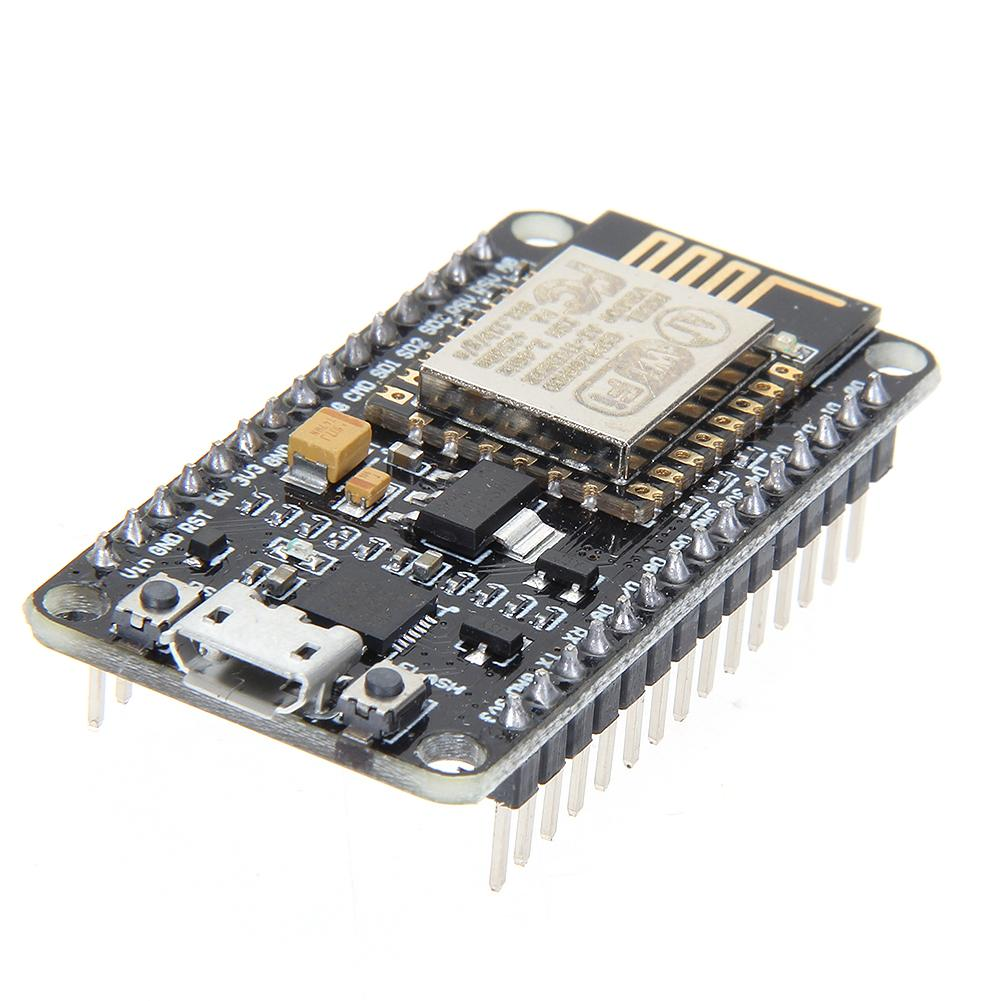
\includegraphics[scale=.1]{esp8266}
	\caption*{\footnotesize{Quelle: \mycite{esp8266}}}
	\label{fig:esp8266}
\end{wrapfigure}

\subsubsection{Nachteile}

\myfootcite[Vgl.][]{hass_vision}
% beispiel vorteile nachteile

\subsection{Monetarisierung}

\subsubsection{Geräte verkaufen} % TODO better title

\subsubsection{Cloud anbieten für IoT Verwaltung} % TODO better title

\subsubsection{Daten verkaufen}% TODO better title

\section{Fazit}

% trends --> closed source, iot :/, automations! :D
% best business cases
% home assistant empfehlung :)